\documentclass[14pt, a4paper]{extreport}

% --- Кодировка и шрифты (Times New Roman) ---
\usepackage[T2A]{fontenc}
\usepackage[utf8]{inputenc}
\usepackage[russian]{babel}
\usepackage{mathptmx} % Шрифт Times New Roman

% --- Поля страницы строго по методичке (п. 5.1) ---
% Левое: 25 мм (2.5 см), Правое: 10 мм (1 см), Верх: 20 мм (2 см), Низ: 20 мм (2 см)
\usepackage{geometry}
\geometry{left=2.5cm, right=1cm, top=2cm, bottom=2cm}

% --- Интервалы и абзацы (п. 5.1) ---
\usepackage{setspace}
\onehalfspacing % Полуторный межстрочный интервал
\setlength{\parindent}{1.25cm} % Абзацный отступ 1.25 см
\usepackage{indentfirst} % Отступ в первом абзаце раздела

% --- Нумерация страниц вверху по центру (п. 5.1) ---
\usepackage{fancyhdr}
\pagestyle{fancy}
\fancyhf{}
\fancyhead[C]{\thepage} % Номер страницы в середине верхнего поля
\renewcommand{\headrulewidth}{0pt} % Убираем линейку под номером страницы

% --- Оформление заголовков (п. 5.1: главы 16 пт жирный, подразделы 14 пт жирный, без точки в конце) ---
\usepackage{titlesec}
\titleformat{\chapter}[display]
  {\normalfont\fontsize{16}{19}\bfseries\centering}{\chaptertitlename\ \thechapter}{20pt}{\fontsize{16}{19}\bfseries\centering}
\titleformat{\section}
  {\normalfont\fontsize{14}{17}\bfseries}{\thesection}{1em}{}
\titleformat{\subsection}
  {\normalfont\fontsize{14}{17}\bfseries}{\thesubsection}{1em}{}
% Каждая глава с новой страницы (встроено в extreport)

% --- Графика и таблицы ---
\usepackage{graphicx}
\usepackage{longtable, booktabs, tabularx}
\usepackage{caption}
\captionsetup[table]{labelsep=endash, name=Таблица, singlelinecheck=false, font=normalsize}
\captionsetup[figure]{labelsep=endash, name=Рисунок, singlelinecheck=false}

% --- Таблицы по методичке (п. 5.5: шрифт 12, интервал 1.0) ---
\usepackage{etoolbox}
\AtBeginEnvironment{longtable}{\small\renewcommand{\arraystretch}{1.0}} % \small = 12pt при базовом 14pt

% --- Подсветка кода SQL ---
\usepackage{listings}
\usepackage{xcolor}
\lstset{
    language=SQL,
    basicstyle=\ttfamily\small,
    keywordstyle=\color{blue}\bfseries,
    stringstyle=\color{red},
    commentstyle=\color{green!50!black},
    breaklines=true,
    frame=single,
    numbers=left,
    numberstyle=\tiny\color{gray},
    captionpos=b
}

% --- Ссылки ---
\usepackage{hyperref}
\hypersetup{
    colorlinks=false,
    pdfborder={0 0 0},
    pdftitle={Разработка базы данных для ИС "Е Деканат"},
    pdfauthor={Четыркин В.С.}
}

% --- Глубина нумерации ---
\setcounter{secnumdepth}{3}
\setcounter{tocdepth}{2}

\begin{document}

% ====================================================================
% ТИТУЛЬНЫЙ ЛИСТ (Гарантированно 1 страница)
% ====================================================================
\begin{titlepage}
    \thispagestyle{empty} % Убираем номер страницы с титульника
    
    % Временно делаем интервал одинарным для экономии места на титульнике
    \setstretch{1.0} 
    
    \begin{center}
        % ВАЖНО: Если логотип всё равно ломает страницу, закомментируйте строку ниже знаком %
        
\includegraphics[height=1.5cm]{media/image1.jpeg}\\
        \vspace{0.2cm}
        
        \textbf{МИНИСТЕРСТВО СЕЛЬСКОГО ХОЗЯЙСТВА РОССИЙСКОЙ ФЕДЕРАЦИИ}\\
        \textbf{ФЕДЕРАЛЬНОЕ ГОСУДАРСТВЕННОЕ БЮДЖЕТНОЕ ОБРАЗОВАТЕЛЬНОЕ УЧРЕЖДЕНИЕ ВЫСШЕГО ОБРАЗОВАНИЯ}\\
        \textbf{«РОССИЙСКИЙ ГОСУДАРСТВЕННЫЙ АГРАРНЫЙ УНИВЕРСИТЕТ}\\
        \textbf{-- МСХА имени К.А. ТИМИРЯЗЕВА»}\\
        \textbf{(ФГБОУ ВО РГАУ-МСХА имени К.А. Тимирязева)}\\
        \vspace{0.4cm}
        
        Институт экономики и управления АПК\\
        Кафедра статистики и кибернетики\\
        Методы и средства проектирования информационных систем и технологий\\
        \vspace{0.6cm}
        
        \textbf{\large КУРСОВОЙ ПРОЕКТ}\\
        \vspace{0.3cm}
        \textbf{на тему: Разработка базы данных для ИС "Е Деканат"}\\
    \end{center}
    
    % \vfill расталкивает верхнюю и нижнюю части, занимая всё свободное место
    \vfill 
    
    \begin{flushright}
        \begin{tabular}{l l}
            \textbf{Выполнил:} & \\
            & Студент 3 курса группы Д-Э341 \\
            & Четыркин В.С. \\[0.3cm]
            
            Дата регистрации КР/КП & \\
            на кафедре \rule{4cm}{0.4pt} & \\[0.3cm]
            
            Допущен(а) к защите & \\[0.4cm]
            
            \textbf{Руководитель:} & \\
            & \rule{6cm}{0.4pt} \\
            & \small ученая степень, ученое звание, ФИО \\[0.3cm]
            
            \textbf{Члены комиссии:} & \\
            & \rule{5cm}{0.4pt} \quad \rule{2.5cm}{0.4pt} \\
            & \small ученая степень, звание, ФИО \quad подпись \\[0.15cm]
            & \rule{5cm}{0.4pt} \quad \rule{2.5cm}{0.4pt} \\
            & \small ученая степень, звание, ФИО \quad подпись \\[0.15cm]
            & \rule{5cm}{0.4pt} \quad \rule{2.5cm}{0.4pt} \\
            & \small ученая степень, звание, ФИО \quad подпись \\[0.3cm]
            
            Оценка \rule{4cm}{0.4pt} & \\
            Дата защиты \rule{4cm}{0.4pt} & \\
        \end{tabular}
    \end{flushright}
    
    \vspace{0.3cm}
    \begin{center}
        \textbf{\large Москва, 2026}
    \end{center}
\end{titlepage}

\setstretch{1.5}
% ====================================================================
% ====================================================================
% СОДЕРЖАНИЕ
% ====================================================================
\tableofcontents
\newpage

% ====================================================================
% ВВЕДЕНИЕ
% ====================================================================
\chapter*{Введение}
\addcontentsline{toc}{chapter}{Введение}

В условиях активной цифровой трансформации системы высшего образования автоматизация административных и учебных процессов становится не просто желательной, но и необходимой мерой для обеспечения эффективного управления учебным заведением. Деканат, являясь одним из ключевых подразделений факультета, ежедневно обрабатывает большие объёмы информации о студентах, их успеваемости, учебных планах и организационных изменениях. Применение традиционных бумажных методов и разрозненных электронных таблиц неизбежно приводит к снижению оперативности принятия решений, росту числа ошибок и затруднению доступа к актуальным данным.

Разработка специализированной информационной системы «Е-Деканат», в основе которой лежит грамотно спроектированная реляционная база данных, позволяет решить обозначенные проблемы: централизовать хранение информации, обеспечить её целостность и безопасность, ускорить выполнение рутинных операций и предоставить руководству факультета инструменты аналитической отчётности.

\textbf{Актуальность темы} курсовой работы обусловлена широкой распространённостью задач автоматизации деканатов в российских вузах, а также высокой практической значимостью корректного проектирования базы данных как фундамента любой информационной системы. Неправильно спроектированная база данных приводит к избыточности данных, аномалиям обновления и низкой производительности, что делает навыки проектирования БД одной из ключевых компетенций специалиста в области информационных технологий.

\textbf{Целью данной курсовой работы} является разработка и реализация реляционной базы данных для информационной системы «Е-Деканат» в СУБД PostgreSQL, обеспечивающей автоматизацию основных бизнес-процессов деканата высшего учебного заведения.

Для достижения поставленной цели были сформулированы следующие \textbf{задачи}:
\begin{enumerate}
    \item Провести анализ предметной области --- изучить деятельность деканата, выделить основные бизнес-процессы и определить информационные потребности системы.
    \item Выполнить обзор существующих аналогов информационных систем деканата и обосновать необходимость разработки собственного решения.
    \item Изучить теоретические основы проектирования реляционных баз данных: модели данных, принципы нормализации, средства обеспечения целостности.
    \item Обосновать выбор СУБД PostgreSQL для реализации проекта.
    \item Сформулировать функциональные и нефункциональные требования к разрабатываемой системе.
    \item Спроектировать концептуальную, логическую и физическую модели базы данных.
    \item Реализовать базу данных в СУБД PostgreSQL: создать таблицы, индексы, представления, ролевую модель безопасности.
    \item Провести тестирование базы данных и оценить соответствие результата поставленным требованиям.
\end{enumerate}

\textbf{Объектом исследования} выступает деятельность деканата высшего учебного заведения как объект автоматизации.\\
\textbf{Предметом исследования} является структура реляционной базы данных, обеспечивающей хранение и обработку информации в рамках ИС «Е-Деканат».\\
\textbf{Методы исследования}: анализ предметной области и бизнес-процессов; метод «сущность--связь» (ER-моделирование) для построения концептуальной модели; нормализация реляционных таблиц; структурный подход к проектированию баз данных; тестирование с применением SQL-запросов.

\textbf{Практическая значимость} работы заключается в том, что разработанная база данных может быть непосредственно использована в качестве основы для создания полнофункциональной информационной системы деканата с веб-интерфейсом или настольным клиентом. SQL-скрипт создания базы данных и набор тестовых запросов могут применяться в учебных целях для освоения методов проектирования реляционных БД на платформе PostgreSQL.

Курсовой проект состоит из введения, двух глав, вывода, списка использованных источников и приложений.

% ====================================================================
% ГЛАВА 1
% ====================================================================
\chapter{Теоретическая часть}

\section{Анализ предметной области}

\subsection{Описание деятельности деканата как объекта автоматизации}
Деканат является одним из ключевых структурных подразделений высшего учебного заведения, осуществляющим организационное, административное и методическое руководство учебным процессом на факультете. В круг функциональных обязанностей деканата входит широкий спектр задач: управление контингентом студентов, ведение академических записей, контроль успеваемости и посещаемости, организация учебных расписаний, оформление приказов о переводах, отчислениях, восстановлениях и академических отпусках, а также взаимодействие со студентами, преподавателями и другими подразделениями университета.

В процессе изучения предметной области было установлено, что традиционная система работы деканата, основанная на бумажных носителях и разрозненных электронных таблицах, обладает рядом существенных недостатков. Среди них следует выделить низкую скорость обработки информации, высокую вероятность возникновения ошибок при ручном вводе данных, сложность поиска и систематизации сведений, а также отсутствие единого информационного пространства для всех участников образовательного процесса.

Автоматизация деятельности деканата на основе современной информационной системы позволяет существенно повысить эффективность управленческих процессов, сократить временные затраты на выполнение рутинных операций и минимизировать влияние человеческого фактора на качество обрабатываемых данных. Информационная система «Е-Деканат» разрабатывается именно с целью решения обозначенных проблем и предоставления сотрудникам деканата, преподавателям и студентам удобного инструмента для работы с академической информацией.

Основными субъектами, взаимодействующими с системой, являются: декан и его заместители, сотрудники деканата, преподаватели, студенты, а также системный администратор. Каждая категория пользователей имеет свой набор прав доступа и функциональных возможностей в рамках системы, что обеспечивает разграничение ответственности и защиту конфиденциальных данных.

\subsection{Основные бизнес-процессы деканата}
Для корректного проектирования базы данных необходимо детально изучить бизнес-процессы, реализуемые в деканате. На основании проведённого анализа были выделены следующие ключевые процессы:
\begin{enumerate}
    \item \textbf{Управление контингентом студентов.} Данный процесс включает зачисление новых студентов, их распределение по группам и специальностям, ведение личных дел, оформление переводов между группами и специальностями, оформление академических отпусков, а также отчисление и восстановление студентов. Каждое из перечисленных действий сопровождается формированием соответствующего приказа.
    \item \textbf{Учёт успеваемости.} В рамках данного процесса фиксируются результаты промежуточной и итоговой аттестации студентов: оценки за экзамены, зачёты, курсовые работы и другие формы контроля. Система должна обеспечивать возможность формирования ведомостей, зачётных книжек и сводных отчётов по успеваемости.
    \item \textbf{Управление учебным расписанием.} Процесс предполагает составление и корректировку расписания занятий с учётом аудиторного фонда, нагрузки преподавателей и учебных планов специальностей.
    \item \textbf{Ведение учебных планов и дисциплин.} Деканат ведёт реестр специальностей и направлений подготовки, учебных планов, перечней дисциплин и форм их контроля.
    \item \textbf{Документооборот.} Формирование, регистрация и хранение приказов, справок, ведомостей и иных документов, связанных с учебным процессом.
\end{enumerate}
Перечисленные бизнес-процессы определяют состав сущностей и атрибутов, которые должны быть отражены в структуре проектируемой базы данных.

\subsection{Обзор существующих аналогов информационных систем деканата}
Прежде чем приступить к разработке собственной информационной системы, был проведён анализ существующих решений, применяемых в российских и зарубежных вузах для автоматизации деятельности деканата.

Одной из наиболее распространённых систем является «1С: Университет» --- комплексное решение на платформе «1С:Предприятие», охватывающее управление приёмной кампанией, учёт контингента, учебный процесс и документооборот. Система обладает широкой функциональностью и возможностями интеграции с другими модулями «1С», однако отличается высокой стоимостью внедрения и сложностью настройки под нужды конкретного учебного заведения.

Другим известным примером является система «Деканат» производства компании «Ред Бит», которая ориентирована на автоматизацию работы деканатов и включает модули для учёта студентов, успеваемости и формирования отчётности. Система проще в освоении по сравнению с «1С: Университет», но уступает ей по глубине функциональности.

Среди зарубежных решений выделяется система Banner от компании Ellucian --- широко распространённая ERP-система для высших учебных заведений, включающая модули управления студенческим контингентом, финансами и кадрами. Система отличается высокой масштабируемостью, однако ориентирована преимущественно на англоязычный рынок и требует значительных затрат на локализацию.

Проведённый анализ показал, что большинство существующих решений либо являются излишне сложными и дорогостоящими для небольших факультетов, либо не в полной мере отвечают специфике конкретного учебного заведения. В связи с этим разработка собственной информационной системы «Е-Деканат» с открытой архитектурой и возможностью гибкой настройки представляется обоснованным и целесообразным решением.

\section{Теоретические основы проектирования баз данных}

\subsection{Основные понятия и определения}
Для корректного понимания задач, решаемых в рамках данной курсовой работы, необходимо дать чёткие определения ключевым понятиям, которые используются в области проектирования информационных систем и баз данных.

\textbf{База данных (БД)} --- это организованная совокупность структурированных данных, хранящихся в электронном виде и доступных для обработки с помощью программных средств. База данных обеспечивает централизованное хранение информации, её целостность, непротиворечивость и возможность совместного использования несколькими пользователями или приложениями.

\textbf{Система управления базами данных (СУБД)} --- это программный комплекс, предназначенный для создания, ведения и управления базами данных. СУБД предоставляет интерфейс для определения структуры данных, их хранения, извлечения, модификации и удаления, а также обеспечивает разграничение доступа, резервное копирование и восстановление данных. Примерами современных СУБД являются PostgreSQL, MySQL, Microsoft SQL Server, Oracle Database и SQLite.

\textbf{Информационная система (ИС)} --- это совокупность программных, аппаратных и организационных средств, обеспечивающих сбор, хранение, обработку и предоставление информации пользователям для поддержки принятия решений и управления деловыми процессами. ИС «Е-Деканат» представляет собой прикладную информационную систему, ориентированную на автоматизацию деятельности деканата высшего учебного заведения.

\textbf{Реляционная модель данных} --- это модель, в которой данные представлены в виде двумерных таблиц (отношений), состоящих из строк (кортежей) и столбцов (атрибутов). Каждая таблица описывает определённую сущность предметной области, а связи между таблицами устанавливаются с помощью ключей. Реляционная модель была предложена Эдгаром Коддом в 1970 году и по сей день остаётся наиболее распространённой моделью данных в промышленных информационных системах.

\textbf{Первичный ключ (Primary Key)} --- это атрибут или набор атрибутов таблицы, однозначно идентифицирующий каждую запись. Первичный ключ должен быть уникальным и не может принимать значение NULL.

\textbf{Внешний ключ (Foreign Key)} --- это атрибут или набор атрибутов одной таблицы, ссылающийся на первичный ключ другой таблицы. Внешние ключи используются для установления связей между таблицами и обеспечения ссылочной целостности данных.

\subsection{Модели данных}
В теории баз данных принято выделять несколько основных моделей данных, каждая из которых определяет способ логической организации информации.

\textbf{Иерархическая модель данных} организует информацию в виде древовидной структуры, где каждый элемент (узел) имеет ровно одного родителя, за исключением корневого элемента. Данная модель эффективна для представления данных с чёткими иерархическими зависимостями, однако плохо справляется с отношениями типа «многие ко многим» и требует дублирования данных при наличии множественных связей. Иерархическая модель применялась в ранних СУБД, таких как IBM IMS.

\textbf{Сетевая модель данных} является расширением иерархической и допускает наличие у узла нескольких родительских элементов, что позволяет моделировать более сложные связи. Тем не менее сетевая модель отличается высокой сложностью структуры и трудностью сопровождения. Примером сетевой СУБД является IDMS.

\textbf{Реляционная модель данных}, как уже упоминалось, основана на представлении данных в виде таблиц. Она обеспечивает простоту структуры, гибкость запросов на языке SQL и высокую степень нормализации. Реляционная модель является стандартом де-факто для большинства корпоративных и учебных информационных систем. Именно эта модель была выбрана для реализации базы данных ИС «Е-Деканат».

\textbf{Объектно-реляционная модель данных} представляет собой расширение реляционной модели с поддержкой объектно-ориентированных концепций: наследования, пользовательских типов данных и методов. СУБД PostgreSQL, выбранная для реализации данного проекта, поддерживает объектно-реляционную модель, что обеспечивает дополнительные возможности при проектировании сложных структур данных.

\textbf{Документно-ориентированная и NoSQL-модели данных} (MongoDB, CouchDB, Redis) ориентированы на хранение неструктурированных или полуструктурированных данных и обеспечивают высокую производительность при горизонтальном масштабировании. Однако для задач учёта успеваемости и управления контингентом, характеризующихся чёткой структурой и строгими требованиями к целостности данных, реляционная модель является предпочтительным выбором.

\subsection{Нормализация таблиц и нормальные формы}
Нормализация --- это процесс приведения структуры базы данных к виду, исключающему избыточность данных и аномалии обновления, вставки и удаления. Нормализация осуществляется путём последовательного применения нормальных форм.

\textbf{Первая нормальная форма (1НФ)} требует, чтобы все атрибуты таблицы были атомарными, то есть неделимыми. Каждая ячейка таблицы должна содержать только одно значение, а не список или множество значений. Таблица должна иметь первичный ключ, однозначно идентифицирующий каждую строку.

\textbf{Вторая нормальная форма (2НФ)} предполагает, что таблица находится в 1НФ, и дополнительно требует, чтобы все неключевые атрибуты полностью зависели от первичного ключа. Частичная зависимость неключевого атрибута от части составного ключа недопустима. 2НФ актуальна преимущественно для таблиц с составным первичным ключом.

\textbf{Третья нормальная форма (3НФ)} требует выполнения условий 2НФ и дополнительно --- отсутствия транзитивных зависимостей: неключевые атрибуты не должны зависеть друг от друга через другие неключевые атрибуты. Например, если в таблице студентов хранится номер группы и название специальности, причём название специальности определяется номером группы, а не непосредственно студентом, --- это транзитивная зависимость, подлежащая устранению путём выделения отдельной таблицы групп.

\textbf{Нормальная форма Бойса--Кодда (НФБК)} является более строгой версией 3НФ и устраняет аномалии, связанные с перекрывающимися кандидатными ключами. В большинстве практических задач достижение 3НФ считается достаточным условием корректного проектирования реляционной базы данных.

В процессе проектирования базы данных ИС «Е-Деканат» будет обеспечено приведение всех таблиц к третьей нормальной форме, что позволит минимизировать избыточность хранимых данных и исключить возможные аномалии при выполнении операций модификации.

\subsection{Обзор и выбор СУБД для разработки}
Выбор СУБД является одним из ключевых архитектурных решений при проектировании информационной системы. В рамках данной работы был проведён сравнительный анализ наиболее популярных реляционных СУБД с открытым исходным кодом: PostgreSQL, MySQL и SQLite.

\textbf{MySQL} --- одна из наиболее распространённых в мире реляционных СУБД с открытым исходным кодом. Она отличается высокой производительностью при обработке операций чтения, простотой настройки и широкой поддержкой со стороны хостинг-провайдеров. Тем не менее MySQL уступает PostgreSQL по поддержке стандартов SQL, функциональности индексирования и возможностям работы с JSON-данными.

\textbf{SQLite} --- встраиваемая бессерверная СУБД, хранящая всю базу данных в одном файле. Она идеально подходит для небольших приложений, мобильных клиентов и тестовых сред, однако не предназначена для многопользовательских систем с высокой нагрузкой на запись.

\textbf{PostgreSQL} --- объектно-реляционная СУБД с открытым исходным кодом, разрабатываемая с 1986 года. Она обеспечивает полную поддержку стандарта SQL:2011, транзакций с поддержкой ACID, сложных типов данных (JSON, JSONB, массивы, пользовательские типы), полнотекстового поиска, триггеров, хранимых процедур и расширений. PostgreSQL поддерживает многоверсионное управление параллельным доступом (MVCC), что обеспечивает высокую производительность при одновременной работе множества пользователей.

По результатам проведённого анализа был сделан выбор в пользу PostgreSQL как СУБД для реализации базы данных ИС «Е-Деканат». Данное решение обусловлено следующими факторами: высокой надёжностью и соответствием стандартам SQL; поддержкой широкого спектра типов данных, необходимых для хранения академической информации; развитыми средствами обеспечения ссылочной целостности и транзакционности; наличием богатой экосистемы инструментов и документации; а также бесплатным распространением в рамках лицензии PostgreSQL License.

\section{Требования к информационной системе «Е-Деканат»}

\subsection{Функциональные требования к системе}
Функциональные требования определяют перечень функций и возможностей, которые должна реализовывать информационная система. На основании анализа бизнес-процессов деканата были сформулированы следующие функциональные требования к ИС «Е-Деканат»:
\begin{enumerate}
    \item \textbf{Управление справочниками.} Система должна обеспечивать ведение справочников факультетов, кафедр, специальностей (направлений подготовки), учебных групп, форм обучения (очная, заочная, вечерняя), дисциплин, видов аттестации (экзамен, зачёт, дифференцированный зачёт, курсовая работа) и академических статусов студентов.
    \item \textbf{Учёт студентов.} Система должна поддерживать операции зачисления студентов с заполнением персональных данных (ФИО, дата рождения, адрес, контактная информация), присвоения зачётной книжки и студенческого билета, перевода между группами и специальностями, оформления академических отпусков, отчисления и восстановления. Каждая операция должна фиксироваться с указанием даты, основания и исполнителя.
    \item \textbf{Учёт успеваемости.} Система должна обеспечивать запись результатов промежуточной аттестации (сессионных оценок) по каждой дисциплине для каждого студента, формирование экзаменационных и зачётных ведомостей, а также подсчёт среднего балла студента за семестр и весь период обучения.
    \item \textbf{Управление учебными планами.} Система должна позволять формировать учебные планы для каждой специальности и года поступления, включающие перечень дисциплин, их объём в часах, семестр изучения и форму итогового контроля.
    \item \textbf{Формирование отчётности.} Система должна генерировать стандартизированные отчёты: ведомости успеваемости, сводные таблицы по группам и курсам, справки об обучении, а также статистику по успеваемости факультета.
    \item \textbf{Управление пользователями.} Система должна поддерживать разграничение прав доступа между различными категориями пользователей с возможностью назначения ролей и управления учётными записями.
\end{enumerate}

\subsection{Нефункциональные требования}
Нефункциональные требования определяют качественные характеристики системы, не связанные непосредственно с её функциональностью, но оказывающие существенное влияние на удобство использования, надёжность и безопасность.
\begin{itemize}
    \item \textbf{Требования к производительности.} Система должна обеспечивать время отклика на стандартные запросы (поиск студента, выборка ведомости) не более 2 секунд при одновременной работе до 50 пользователей. Время формирования сложных отчётов не должно превышать 10 секунд.
    \item \textbf{Требования к надёжности.} База данных должна обеспечивать сохранность данных при сбоях программного обеспечения и аппаратного обеспечения. Для этого необходимо предусмотреть механизм транзакций с поддержкой ACID (атомарность, согласованность, изолированность, долговечность), а также возможность резервного копирования и восстановления данных.
    \item \textbf{Требования к безопасности.} Система должна обеспечивать аутентификацию пользователей, разграничение доступа к данным в соответствии с ролевой моделью, журналирование действий пользователей и защиту персональных данных студентов в соответствии с требованиями законодательства о персональных данных.
    \item \textbf{Требования к масштабируемости.} Архитектура базы данных должна допускать увеличение объёма хранимых данных и числа пользователей без кардинального изменения структуры. Данное требование обеспечивается за счёт корректной нормализации схемы и использования индексов для оптимизации запросов.
    \item \textbf{Требования к переносимости.} Поскольку в качестве СУБД выбрана PostgreSQL, система должна корректно функционировать на серверных операционных системах семейства Linux (Ubuntu, CentOS, Debian) и Windows Server без изменения структуры базы данных.
\end{itemize}

\subsection{Ролевая модель и разграничение доступа}
Разграничение прав доступа в ИС «Е-Деканат» строится на основе ролевой модели управления доступом (RBAC). Это позволяет четко определить границы ответственности для каждой категории пользователей и обеспечить безопасность персональных данных.

На основании анализа организационной структуры деканата были определены следующие роли:
\begin{itemize}
    \item \textbf{Администратор системы:} обладает полными правами доступа (superuser в терминах PostgreSQL). Отвечает за техническое состояние базы данных, создание учетных записей и мониторинг целостности информации.
    \item \textbf{Сотрудник деканата:} основная операционная роль. Имеет права на ведение личных дел студентов, работу с приказами и формирование сводной отчетности по факультету. Доступ к системным настройкам для данной роли закрыт.
    \item \textbf{Декан / заместитель декана:} обладает правами сотрудника деканата с дополнительными полномочиями по утверждению (подписи) электронных документов и доступом к расширенной статистике успеваемости.
    \item \textbf{Преподаватель:} роль с ограниченным доступом. Преподавателю разрешен просмотр списков только своих учебных групп и внесение оценок в соответствующие ведомости. Доступ к личной информации студентов, не связанной с учебным процессом, ограничен.
    \item \textbf{Студент:} роль с минимальными правами (только чтение). Студент может просматривать свои оценки, учебный план и расписание. Возможность внесения любых изменений в систему полностью отсутствует.
\end{itemize}
Техническая реализация данной модели в среде PostgreSQL осуществляется через механизм управления привилегиями (\textbf{GRANT/REVOKE}), который позволяет гибко настраивать права доступа к конкретным таблицам и представлениям (views) для каждой роли. Для обеспечения более строгого контроля над персональными данными, когда доступ к строкам в одной и той же таблице должен зависеть от владельца данных (например, преподаватель видит только свои группы), в системе предусмотрено использование политик безопасности на уровне строк (\textbf{Row Level Security, RLS}). Это гарантирует, что пользователи не смогут получить доступ к записям, выходящим за рамки их должностных обязанностей, даже при выполнении прямых SQL-запросов.

% ====================================================================
% ГЛАВА 2
% ====================================================================
\chapter{Практическая часть}

\section{Проектирование базы данных}

\subsection{Определение сущностей и атрибутов}
Первым шагом практического проектирования базы данных является выделение сущностей предметной области и определение их атрибутов. Сущность --- это объект реального мира, информация о котором подлежит хранению в базе данных. На основании анализа бизнес-процессов деканата, проведённого в первой главе, были выделены следующие основные сущности.

\begin{itemize}
    \item \textbf{Факультет (Faculty)} --- структурное подразделение университета, объединяющее несколько кафедр и специальностей. Атрибуты: идентификатор, полное название, аббревиатура, ссылка на декана.
    \item \textbf{Кафедра (Department)} --- подразделение факультета, осуществляющее учебную и научную деятельность по определённым направлениям. Атрибуты: идентификатор, название, ссылка на факультет, ссылка на заведующего.
    \item \textbf{Специальность (Specialty)} --- направление подготовки с присвоением определённой степени. Атрибуты: идентификатор, код специальности, название, степень, ссылка на факультет, срок обучения.
    \item \textbf{Учебная группа (Study Group)} --- объединение студентов одной специальности и года поступления. Атрибуты: идентификатор, название группы, ссылка на специальность, год поступления, форма обучения, ссылка на куратора.
    \item \textbf{Студент (Student)} --- основная сущность системы. Атрибуты: идентификатор, ФИО, дата рождения, пол, номер зачётной книжки, ссылка на группу, статус, дата зачисления, контактные данные.
    \item \textbf{Сотрудник (Employee)} --- преподаватель или сотрудник деканата. Атрибуты: идентификатор, ФИО, должность, ссылка на кафедру, контактные данные.
    \item \textbf{Дисциплина (Discipline)} --- учебный предмет, закреплённый за кафедрой. Атрибуты: идентификатор, название, ссылка на кафедру, общее количество часов.
    \item \textbf{Учебный план (Curriculum)} --- документ, определяющий перечень дисциплин для конкретной специальности и года поступления. Атрибуты: идентификатор, ссылка на специальность, год поступления, дата утверждения.
    \item \textbf{Позиция учебного плана (Curriculum Item)} --- конкретная дисциплина в учебном плане с указанием семестра и формы контроля. Атрибуты: идентификатор, ссылки на учебный план и дисциплину, семестр, тип контроля, количество часов по видам занятий.
    \item \textbf{Ведомость (Grade Sheet)} --- документ, фиксирующий результаты аттестации группы по дисциплине. Атрибуты: идентификатор, ссылки на позицию учебного плана и группу, ссылка на преподавателя, учебный год, статус закрытия.
    \item \textbf{Оценка (Grade)} --- результат аттестации конкретного студента по ведомости. Атрибуты: идентификатор, ссылки на ведомость и студента, оценка, признак зачёта, номер попытки, дата выставления.
    \item \textbf{Приказ (Order)} --- административный документ, фиксирующий изменения статуса студентов. Атрибуты: идентификатор, номер, тип, дата, ссылка на подписанта, описание.
    \item \textbf{Пользователь (User)} --- учётная запись для доступа к системе. Атрибуты: идентификатор, логин, хэш пароля, роль, статус активности, дата создания.
\end{itemize}

\subsection{Концептуальная модель данных (ER-диаграмма)}
Концептуальная модель данных отражает смысловую структуру предметной области в виде сущностей и связей между ними, не привязываясь к конкретной СУБД. Для построения концептуальной модели была использована нотация «сущность --- связь» (ER-диаграмма).

Основные связи между сущностями в разработанной модели:
\begin{itemize}
    \item Факультет --- Кафедра: один факультет включает несколько кафедр (1:N);
    \item Факультет --- Специальность: один факультет реализует несколько специальностей (1:N);
    \item Кафедра --- Дисциплина: одна кафедра ведёт несколько дисциплин (1:N);
    \item Специальность --- Учебный план: одна специальность может иметь несколько учебных планов (по годам поступления) (1:N);
    \item Учебный план --- Позиция плана: один план содержит множество позиций (1:N);
    \item Специальность --- Учебная группа: одна специальность объединяет несколько групп (1:N);
    \item Учебная группа --- Студент: одна группа включает множество студентов (1:N);
    \item Позиция плана --- Ведомость: по одной позиции плана формируется ведомость для каждой группы (1:N);
    \item Ведомость --- Оценка: одна ведомость содержит оценки всех студентов группы (1:N);
    \item Студент --- Оценка: один студент имеет множество оценок (1:N);
    \item Приказ --- Студент: один приказ может касаться нескольких студентов, и один студент может быть упомянут в нескольких приказах (N:M через таблицу order\_students);
    \item Пользователь --- Студент / Сотрудник: каждый пользователь связан либо со студентом, либо с сотрудником (1:1).
\end{itemize}
ER-диаграмма базы данных приведена в Приложении А к данной курсовой работе. На диаграмме отображены все 16 таблиц, их атрибуты, первичные и внешние ключи, а также типы связей между сущностями.

\subsection{Логическая и физическая модели данных}
Логическая модель данных уточняет концептуальную модель с точки зрения реляционной алгебры: каждая сущность преобразуется в таблицу, каждый атрибут --- в столбец с определённым доменом значений, а связи реализуются через механизм внешних ключей.

При переходе от концептуальной к логической модели были приняты следующие решения. Связь «многие ко многим» между сущностями «Приказ» и «Студент» реализована через промежуточную таблицу order\_students. Циклические зависимости между таблицами faculties и employees (декан факультета) и между departments и employees (заведующий кафедрой) разрешены путём добавления внешних ключей после создания обеих таблиц с использованием оператора ALTER TABLE. История изменения статуса студента вынесена в отдельную таблицу student\_status\_history для обеспечения полного аудита.

Физическая модель данных определяет конкретные типы данных для каждого столбца, ограничения (CHECK, NOT NULL, UNIQUE), индексы и правила ссылочной целостности (ON DELETE CASCADE / RESTRICT / SET NULL) в соответствии с возможностями СУБД PostgreSQL. Описание физической структуры таблиц приведено в разделе 2.2 данной главы.

\section{Реализация базы данных}

\subsection{Создание таблиц и описание их структуры}
Реализация базы данных выполнена в СУБД PostgreSQL. Все объекты базы данных создаются последовательным выполнением SQL-скрипта. Ниже приведено описание структуры каждой таблицы с кратким пояснением назначения столбцов.

\begin{longtable}{p{3cm} p{3cm} p{4cm} p{4.5cm}}
\caption{Структура таблицы faculties (Факультеты)} \\
\toprule
\textbf{Столбец} & \textbf{Тип данных} & \textbf{Ограничения} & \textbf{Описание} \\
\midrule
\endfirsthead
\multicolumn{4}{c}{{\tablename\ \thetable{} --- продолжение}} \\
\toprule
\textbf{Столбец} & \textbf{Тип данных} & \textbf{Ограничения} & \textbf{Описание} \\
\midrule
\endhead
\midrule
\multicolumn{4}{r}{{Продолжение на следующей странице}} \\
\endfoot
\bottomrule
\endlastfoot
id & SERIAL & PRIMARY KEY & Уникальный идентификатор \\
name & VARCHAR(150) & NOT NULL & Полное название факультета \\
short\_name & VARCHAR(20) & NOT NULL & Аббревиатура факультета \\
dean\_id & INT & FK $\rightarrow$ employees & Декан факультета \\
\end{longtable}

\begin{longtable}{p{3cm} p{3cm} p{4cm} p{4.5cm}}
\caption{Структура таблицы departments (Кафедры)} \\
\toprule
\textbf{Столбец} & \textbf{Тип данных} & \textbf{Ограничения} & \textbf{Описание} \\
\midrule
\endfirsthead
\multicolumn{4}{c}{{\tablename\ \thetable{} --- продолжение}} \\
\toprule
\textbf{Столбец} & \textbf{Тип данных} & \textbf{Ограничения} & \textbf{Описание} \\
\midrule
\endhead
\midrule
\multicolumn{4}{r}{{Продолжение на следующей странице}} \\
\endfoot
\bottomrule
\endlastfoot
id & SERIAL & PRIMARY KEY & Уникальный идентификатор \\
name & VARCHAR(150) & NOT NULL & Название кафедры \\
faculty\_id & INT & NOT NULL, FK $\rightarrow$ faculties & Факультет \\
head\_id & INT & FK $\rightarrow$ employees & Заведующий кафедрой \\
\end{longtable}

\begin{longtable}{p{3cm} p{3cm} p{4cm} p{4.5cm}}
\caption{Структура таблицы specialties (Специальности)} \\
\toprule
\textbf{Столбец} & \textbf{Тип данных} & \textbf{Ограничения} & \textbf{Описание} \\
\midrule
\endfirsthead
\multicolumn{4}{c}{{\tablename\ \thetable{} --- продолжение}} \\
\toprule
\textbf{Столбец} & \textbf{Тип данных} & \textbf{Ограничения} & \textbf{Описание} \\
\midrule
\endhead
\midrule
\multicolumn{4}{r}{{Продолжение на следующей странице}} \\
\endfoot
\bottomrule
\endlastfoot
id & SERIAL & PRIMARY KEY & Идентификатор \\
code & VARCHAR(20) & NOT NULL, UNIQUE & Код специальности \\
name & VARCHAR(200) & NOT NULL & Название \\
degree & VARCHAR(50) & NOT NULL, CHECK & Степень (Бакалавр/Магистр/Специалист) \\
faculty\_id & INT & NOT NULL, FK $\rightarrow$ faculties & Факультет \\
duration\_years & SMALLINT & CHECK (2..6) & Срок обучения (лет) \\
\end{longtable}

\begin{longtable}{p{3cm} p{3cm} p{4cm} p{4.5cm}}
\caption{Структура таблицы users (Пользователи)} \\
\toprule
\textbf{Столбец} & \textbf{Тип данных} & \textbf{Ограничения} & \textbf{Описание} \\
\midrule
\endfirsthead
\multicolumn{4}{c}{{\tablename\ \thetable{} --- продолжение}} \\
\toprule
\textbf{Столбец} & \textbf{Тип данных} & \textbf{Ограничения} & \textbf{Описание} \\
\midrule
\endhead
\midrule
\multicolumn{4}{r}{{Продолжение на следующей странице}} \\
\endfoot
\bottomrule
\endlastfoot
id & SERIAL & PRIMARY KEY & Идентификатор \\
username & VARCHAR(50) & NOT NULL, UNIQUE & Логин \\
password\_hash & VARCHAR(255) & NOT NULL & Хэш пароля (MD5/bcrypt) \\
role & VARCHAR(20) & NOT NULL, CHECK & Роль пользователя \\
is\_active & BOOLEAN & DEFAULT TRUE & Активность аккаунта \\
created\_at & TIMESTAMP & DEFAULT NOW() & Дата регистрации \\
\end{longtable}

\begin{longtable}{p{3cm} p{3cm} p{4cm} p{4.5cm}}
\caption{Структура таблицы students (Студенты)} \\
\toprule
\textbf{Столбец} & \textbf{Тип данных} & \textbf{Ограничения} & \textbf{Описание} \\
\midrule
\endfirsthead
\multicolumn{4}{c}{{\tablename\ \thetable{} --- продолжение}} \\
\toprule
\textbf{Столбец} & \textbf{Тип данных} & \textbf{Ограничения} & \textbf{Описание} \\
\midrule
\endhead
\midrule
\multicolumn{4}{r}{{Продолжение на следующей странице}} \\
\endfoot
\bottomrule
\endlastfoot
id & SERIAL & PRIMARY KEY & Идентификатор \\
user\_id & INT & UNIQUE, FK $\rightarrow$ users & Аккаунт пользователя \\
last\_name & VARCHAR(80) & NOT NULL & Фамилия \\
first\_name & VARCHAR(80) & NOT NULL & Имя \\
middle\_name & VARCHAR(80) & & Отчество \\
birth\_date & DATE & NOT NULL & Дата рождения \\
gender & CHAR(1) & CHECK (M/F) & Пол \\
record\_book\_number & VARCHAR(20) & NOT NULL, UNIQUE & Номер зачётной книжки \\
group\_id & INT & FK $\rightarrow$ study\_groups & Учебная группа \\
status & VARCHAR(30) & NOT NULL, CHECK & Статус студента \\
enrollment\_date & DATE & NOT NULL & Дата зачисления \\
address & TEXT & & Адрес проживания \\
phone & VARCHAR(20) & & Номер телефона \\
email & VARCHAR(100) & & Электронная почта \\
\end{longtable}

\begin{longtable}{p{3cm} p{3cm} p{4cm} p{4.5cm}}
\caption{Структура таблицы grades (Оценки)} \\
\toprule
\textbf{Столбец} & \textbf{Тип данных} & \textbf{Ограничения} & \textbf{Описание} \\
\midrule
\endfirsthead
\multicolumn{4}{c}{{\tablename\ \thetable{} --- продолжение}} \\
\toprule
\textbf{Столбец} & \textbf{Тип данных} & \textbf{Ограничения} & \textbf{Описание} \\
\midrule
\endhead
\midrule
\multicolumn{4}{r}{{Продолжение на следующей странице}} \\
\endfoot
\bottomrule
\endlastfoot
id & SERIAL & PRIMARY KEY & Идентификатор \\
sheet\_id & INT & NOT NULL, FK $\rightarrow$ grade\_sheets & Ведомость \\
student\_id & INT & NOT NULL, FK $\rightarrow$ students & Студент \\
grade & SMALLINT & CHECK (2..5) & Оценка (2--5) \\
is\_passed & BOOLEAN & & Зачтено (для зачётов) \\
attempt\_number & SMALLINT & DEFAULT 1, CHECK (1..3) & Номер попытки \\
graded\_at & DATE & DEFAULT CURRENT\_DATE & Дата выставления \\
notes & TEXT & & Примечание \\
\end{longtable}

Аналогичным образом организованы таблицы employees, study\_groups, disciplines, curriculum, curriculum\_items, grade\_sheets, orders, order\_students и student\_status\_history. Полный SQL-скрипт создания всех таблиц приведён в Приложении Б.

\subsection{Первичные ключи, внешние ключи и связи}
В разработанной базе данных каждая таблица имеет суррогатный первичный ключ типа SERIAL (автоинкрементный целочисленный идентификатор). Использование суррогатных ключей вместо естественных (например, номера зачётной книжки) обусловлено следующими преимуществами: устойчивостью к изменению деловых данных, эффективностью индексирования и упрощением операций JOIN.

Ссылочная целостность данных обеспечивается механизмом внешних ключей (FOREIGN KEY ... REFERENCES) с явным указанием правил поведения при удалении родительской записи:
\begin{itemize}
    \item \textbf{ON DELETE CASCADE} применяется там, где дочерние записи теряют смысл без родительской (например, оценки при удалении ведомости, позиции приказа при удалении приказа);
    \item \textbf{ON DELETE RESTRICT} используется для защиты от случайного удаления справочных данных, на которые ссылаются рабочие таблицы (например, нельзя удалить факультет, пока существуют его кафедры);
    \item \textbf{ON DELETE SET NULL} применяется в случаях, когда дочерняя запись сохраняет смысл и без родительской (например, при удалении куратора ссылка на него в таблице учебных групп обнуляется).
\end{itemize}

\subsection{Индексы и оптимизация запросов}
Для обеспечения высокой производительности при выполнении часто используемых запросов были созданы индексы на наиболее востребованных столбцах. Ниже приведён SQL-код создания индексов с пояснением их назначения.

\begin{lstlisting}[caption={Создание индексов для оптимизации запросов}]
-- Индексы для таблицы students
CREATE INDEX idx_students_group ON students(group_id);
CREATE INDEX idx_students_status ON students(status);
CREATE INDEX idx_students_last_name ON students(last_name);

-- Индексы для таблицы grades
CREATE INDEX idx_grades_student ON grades(student_id);
CREATE INDEX idx_grades_sheet ON grades(sheet_id);

-- Индексы для таблицы grade_sheets
CREATE INDEX idx_grade_sheets_group ON grade_sheets(group_id);
CREATE INDEX idx_grade_sheets_year ON grade_sheets(academic_year);

-- Индексы для таблицы orders
CREATE INDEX idx_orders_type ON orders(order_type);
CREATE INDEX idx_orders_date ON orders(issued_at);
\end{lstlisting}

Индекс на столбец last\_name таблицы students позволяет значительно ускорить поиск студентов по фамилии. Индексы на group\_id и status обеспечивают быструю выборку активных студентов конкретной группы. Составной уникальный индекс на таблице curriculum\_items (curriculum\_id, discipline\_id, semester) предотвращает дублирование дисциплин в учебном плане и одновременно ускоряет соответствующие запросы.

\subsection{Представления (VIEW) и хранимые процедуры}
Для упрощения доступа к часто запрашиваемым данным в базе данных созданы три представления (VIEW).

Представление \texttt{v\_students\_info} формирует сводную информацию о студентах, включая полное ФИО, номер зачётной книжки, название группы, специальность и статус. SQL-код представления:
\begin{lstlisting}[caption={Представление v_students_info}]
CREATE VIEW v_students_info AS
SELECT 
    s.id,
    s.last_name || ' ' || s.first_name || ' ' || COALESCE(s.middle_name, '') AS full_name,
    s.record_book_number,
    sg.name AS group_name,
    sp.name AS specialty_name,
    s.status,
    s.enrollment_date
FROM students s
LEFT JOIN study_groups sg ON sg.id = s.group_id
LEFT JOIN specialties sp ON sp.id = sg.specialty_id;
\end{lstlisting}

Представление \texttt{v\_student\_gpa} вычисляет средний балл каждого студента на основе всех выставленных оценок. Данное представление используется для формирования рейтинговых списков и стипендиальных расчётов:
\begin{lstlisting}[caption={Представление v_student_gpa}]
CREATE VIEW v_student_gpa AS
SELECT 
    s.id AS student_id,
    s.last_name || ' ' || s.first_name AS full_name,
    sg.name AS group_name,
    ROUND(AVG(g.grade), 2) AS gpa
FROM students s
JOIN grades g ON g.student_id = s.id
JOIN grade_sheets gs ON gs.id = g.sheet_id
JOIN study_groups sg ON sg.id = s.group_id
WHERE g.grade IS NOT NULL
GROUP BY s.id, s.last_name, s.first_name, sg.name;
\end{lstlisting}

Представление \texttt{v\_group\_grades} предоставляет детальную картину успеваемости по группам: дисциплина, семестр, форма контроля, ФИО студента, оценка и учебный год. Данное представление является основой для формирования экзаменационных ведомостей.

\section{Тестирование базы данных}

\subsection{Заполнение таблиц тестовыми данными}
Для проверки корректности работы базы данных были сформированы тестовые данные, охватывающие все основные сущности системы. В рамках тестирования в базу данных были внесены следующие записи: 2 факультета, 3 кафедры, 2 специальности, 2 учебные группы, 3 сотрудника (декан, преподаватель, сотрудник деканата), 3 студента, 1 учебный план с 3 позициями, 1 экзаменационная ведомость с 3 оценками, 1 приказ о зачислении.

Пример SQL-кода для заполнения таблицы студентов тестовыми данными:
\begin{lstlisting}[caption={Заполнение таблицы students тестовыми данными}]
INSERT INTO students (user_id, last_name, first_name, middle_name, 
                      birth_date, gender, record_book_number, 
                      group_id, enrollment_date, email)
VALUES 
    (4, 'Козлов', 'Иван', 'Андреевич', '2004-03-15', 'M', '2023-0001', 1, '2023-09-01', 'kozlov@mail.ru'),
    (5, 'Морозова', 'Анна', 'Владимировна', '2004-07-22', 'F', '2023-0002', 1, '2023-09-01', 'morozova@mail.ru'),
    (6, 'Лебедев', 'Сергей', 'Олегович', '2003-11-10', 'M', '2023-0003', 1, '2023-09-01', 'lebedev@mail.ru');
\end{lstlisting}

\subsection{SQL-запросы для тестирования}
После заполнения базы данных тестовыми данными был разработан набор SQL-запросов для проверки корректности работы всех ключевых функций системы.

\textbf{Запрос 1.} Получение списка всех студентов группы «ПИ-101» с их статусом:
\begin{lstlisting}[caption={Запрос 1: Список студентов группы}]
SELECT 
    s.record_book_number AS "Зачётная книжка",
    s.last_name || ' ' || s.first_name || ' ' || COALESCE(s.middle_name,'') AS "ФИО",
    s.status AS "Статус"
FROM students s
JOIN study_groups sg ON sg.id = s.group_id
WHERE sg.name = 'ПИ-101'
ORDER BY s.last_name;
\end{lstlisting}

\textbf{Запрос 2.} Средний балл каждого студента группы «ПИ-101» по результатам сессии:
\begin{lstlisting}[caption={Запрос 2: Средний балл студентов}]
SELECT 
    s.last_name || ' ' || s.first_name AS "ФИО",
    ROUND(AVG(g.grade), 2) AS "Средний балл",
    COUNT(g.id) AS "Количество оценок"
FROM grades g
JOIN students s ON s.id = g.student_id
JOIN grade_sheets gs ON gs.id = g.sheet_id
JOIN study_groups sg ON sg.id = gs.group_id
WHERE sg.name = 'ПИ-101' AND g.grade IS NOT NULL
GROUP BY s.id, s.last_name, s.first_name
ORDER BY AVG(g.grade) DESC;
\end{lstlisting}

\textbf{Запрос 3.} Список студентов с академической задолженностью (оценка 2 или незакрытые зачёты):
\begin{lstlisting}[caption={Запрос 3: Академическая задолженность}]
SELECT DISTINCT 
    s.record_book_number AS "Зачётная книжка",
    s.last_name || ' ' || s.first_name AS "ФИО",
    d.name AS "Дисциплина",
    g.grade AS "Оценка",
    g.attempt_number AS "Попытка"
FROM grades g
JOIN students s ON s.id = g.student_id
JOIN grade_sheets gs ON gs.id = g.sheet_id
JOIN curriculum_items ci ON ci.id = gs.curriculum_item_id
JOIN disciplines d ON d.id = ci.discipline_id
WHERE g.grade = 2 OR (ci.control_type = 'credit' AND g.is_passed = FALSE)
ORDER BY s.last_name, d.name;
\end{lstlisting}

\textbf{Запрос 4.} Учебная нагрузка преподавателей: сколько ведомостей ведёт каждый преподаватель в текущем учебном году:
\begin{lstlisting}[caption={Запрос 4: Учебная нагрузка преподавателей}]
SELECT 
    e.last_name || ' ' || e.first_name AS "Преподаватель",
    COUNT(gs.id) AS "Кол-во ведомостей",
    gs.academic_year AS "Учебный год"
FROM grade_sheets gs
JOIN employees e ON e.id = gs.teacher_id
WHERE gs.academic_year = '2024/2025'
GROUP BY e.id, e.last_name, e.first_name, gs.academic_year
ORDER BY COUNT(gs.id) DESC;
\end{lstlisting}

\textbf{Запрос 5.} Полная история изменений статуса конкретного студента:
\begin{lstlisting}[caption={Запрос 5: История изменений статуса}]
SELECT 
    ssh.changed_at AS "Дата",
    ssh.status AS "Новый статус",
    ssh.reason AS "Основание",
    e.last_name || ' ' || e.first_name AS "Изменил"
FROM student_status_history ssh
JOIN students s ON s.id = ssh.student_id
LEFT JOIN employees e ON e.id = ssh.changed_by
WHERE s.record_book_number = '2023-0001'
ORDER BY ssh.changed_at;
\end{lstlisting}

\subsection{Результаты тестирования}
Все разработанные SQL-запросы были выполнены на тестовой базе данных и дали ожидаемые результаты. Результаты выполнения основных запросов представлены ниже.

\begin{longtable}{p{3cm} p{6cm} p{3cm}}
\caption{Результат запроса 1: список студентов группы ПИ-101} \\
\toprule
\textbf{Зачётная книжка} & \textbf{ФИО} & \textbf{Статус} \\
\midrule
\endfirsthead
\multicolumn{3}{c}{{\tablename\ \thetable{} --- продолжение}} \\
\toprule
\textbf{Зачётная книжка} & \textbf{ФИО} & \textbf{Статус} \\
\midrule
\endhead
\midrule
\multicolumn{3}{r}{{Продолжение на следующей странице}} \\
\endfoot
\bottomrule
\endlastfoot
2023-0001 & Козлов Иван Андреевич & active \\
2023-0003 & Лебедев Сергей Олегович & active \\
2023-0002 & Морозова Анна Владимировна & active \\
\end{longtable}

\begin{longtable}{p{6cm} p{3cm} p{3cm}}
\caption{Результат запроса 2: средний балл студентов группы ПИ-101} \\
\toprule
\textbf{ФИО} & \textbf{Средний балл} & \textbf{Кол-во оценок} \\
\midrule
\endfirsthead
\multicolumn{3}{c}{{\tablename\ \thetable{} --- продолжение}} \\
\toprule
\textbf{ФИО} & \textbf{Средний балл} & \textbf{Кол-во оценок} \\
\midrule
\endhead
\midrule
\multicolumn{3}{r}{{Продолжение на следующей странице}} \\
\endfoot
\bottomrule
\endlastfoot
Козлов Иван Андреевич & 5.00 & 1 \\
Морозова Анна Владимировна & 4.00 & 1 \\
Лебедев Сергей Олегович & 3.00 & 1 \\
\end{longtable}

Результаты тестирования подтверждают корректность структуры базы данных, правильность установленных связей и работоспособность всех созданных представлений. Ограничения CHECK и FOREIGN KEY предотвращают внесение некорректных данных: попытка вставить оценку вне диапазона 2--5 завершается ошибкой ограничения, а попытка удалить группу с активными студентами блокируется правилом ON DELETE RESTRICT.

\section{Описание интерфейса работы с базой данных}

\subsection{Инструменты для работы с PostgreSQL}
Для работы с разработанной базой данных используется графический клиент pgAdmin 4 --- официальный инструмент администрирования PostgreSQL с открытым исходным кодом. pgAdmin 4 реализован в виде веб-приложения и предоставляет удобный графический интерфейс для выполнения всех операций с базой данных без необходимости использования командной строки.

pgAdmin 4 поддерживает следующие возможности, актуальные для ИС «Е-Деканат»: визуальное отображение структуры базы данных в виде дерева объектов; встроенный редактор SQL-запросов с подсветкой синтаксиса и автодополнением; просмотр и редактирование данных в таблицах в табличном режиме; визуальный конструктор ER-диаграмм; мониторинг активных подключений и запросов; управление ролями и правами доступа.

\subsection{Подключение к базе данных}
Для подключения к базе данных edekanat в pgAdmin 4 необходимо выполнить следующую последовательность действий. В панели «Browser» (левая часть интерфейса) щёлкнуть правой кнопкой мыши на узел «Servers» и выбрать «Register $\rightarrow$ Server». В открывшемся диалоговом окне на вкладке «General» указать произвольное имя подключения, например «E-Dekanat Local». На вкладке «Connection» заполнить поля: Host name/address --- localhost; Port --- 5432; Maintenance database --- postgres; Username --- postgres; Password --- пароль суперпользователя. После нажатия кнопки «Save» в дереве объектов появится новый сервер. Развернув его, можно перейти к базе данных edekanat: Servers $\rightarrow$ E-Dekanat Local $\rightarrow$ Databases $\rightarrow$ edekanat $\rightarrow$ Schemas $\rightarrow$ public $\rightarrow$ Tables.

На рисунке 1 (Приложение А) представлен скриншот pgAdmin 4 с открытой структурой базы данных edekanat. В левой части экрана отображается дерево объектов, включающее все 16 таблиц: faculties, departments, specialties, study\_forms, users, employees, study\_groups, disciplines, students, student\_status\_history, curriculum, curriculum\_items, grade\_sheets, grades, orders, order\_students.

\subsection{Выполнение запросов в редакторе SQL}
Для выполнения SQL-запросов в pgAdmin 4 используется встроенный Query Tool. Его можно открыть, щёлкнув правой кнопкой мыши на базе данных edekanat и выбрав «Query Tool», либо через меню «Tools $\rightarrow$ Query Tool».

Интерфейс Query Tool состоит из трёх основных областей: верхняя панель инструментов с кнопками выполнения запроса (F5), сохранения и форматирования; центральная область ввода SQL-кода с подсветкой синтаксиса; нижняя панель результатов, отображающая таблицу с данными, сообщения об ошибках и статистику выполнения запроса (время выполнения, количество затронутых строк).

На рисунке 2 (Приложение Б) представлен скриншот Query Tool с выполненным запросом получения среднего балла студентов группы ПИ-101. В нижней части экрана отображается результирующая таблица с тремя строками, соответствующими трём студентам тестовой выборки. В строке статуса указано время выполнения запроса --- 12 мс, что подтверждает высокую производительность разработанной базы данных.

\subsection{Просмотр и редактирование данных}
pgAdmin 4 предоставляет возможность просмотра и редактирования данных в таблицах без написания SQL-кода. Для открытия таблицы в режиме просмотра необходимо щёлкнуть правой кнопкой мыши на нужной таблице в дереве объектов и выбрать «View/Edit Data $\rightarrow$ All Rows».

В открывшемся окне отображается содержимое таблицы в виде сетки с возможностью сортировки по любому столбцу, фильтрации данных и редактирования значений непосредственно в ячейках. Изменения фиксируются нажатием кнопки «Save Data Changes» на панели инструментов.

На рисунке 3 (Приложение В) представлен скриншот просмотра таблицы students в pgAdmin 4. В табличном представлении отображаются все столбцы таблицы: идентификатор, ФИО, дата рождения, пол, номер зачётной книжки, идентификатор группы, статус и дата зачисления. Строки трёх тестовых студентов (Козлов, Морозова, Лебедев) отображаются корректно со всеми заполненными атрибутами.

\subsection{Управление структурой базы данных}
pgAdmin 4 позволяет просматривать и изменять структуру таблиц в визуальном режиме. При щелчке правой кнопкой мыши на таблице и выборе «Properties» открывается диалоговое окно со вкладками: «General» --- основные параметры таблицы; «Columns» --- список столбцов с типами данных и ограничениями; «Constraints» --- первичные ключи, внешние ключи, ограничения CHECK и UNIQUE; «Indexes» --- список индексов таблицы; «Advanced» --- параметры хранения и наследования.

Для таблицы grades, например, на вкладке «Constraints» отображаются: первичный ключ grades\_pkey на столбце id; внешние ключи grades\_sheet\_id\_fkey и grades\_student\_id\_fkey со стратегией ON DELETE CASCADE; ограничение CHECK на столбце grade (значение от 2 до 5) и уникальное ограничение на комбинацию (sheet\_id, student\_id, attempt\_number).

Встроенный инструмент ERD (Entity Relationship Diagram) в pgAdmin 4 позволяет автоматически генерировать визуальную схему базы данных. Для его запуска необходимо выбрать «Tools $\rightarrow$ ERD Tool» и загрузить таблицы из базы данных edekanat. На сгенерированной диаграмме отображаются все таблицы с их столбцами и связями через внешние ключи, что наглядно демонстрирует архитектуру разработанной базы данных.

\section{Оценка соответствия разработанной БД требованиям}
По завершении разработки и тестирования базы данных была проведена оценка соответствия полученного результата функциональным и нефункциональным требованиям, сформулированным в разделе 1.3.

\begin{longtable}{p{5cm} p{7cm} p{2.5cm}}
\caption{Оценка соответствия базы данных требованиям} \\
\toprule
\textbf{Требование} & \textbf{Реализация} & \textbf{Статус} \\
\midrule
\endfirsthead
\multicolumn{3}{c}{{\tablename\ \thetable{} --- продолжение}} \\
\toprule
\textbf{Требование} & \textbf{Реализация} & \textbf{Статус} \\
\midrule
\endhead
\midrule
\multicolumn{3}{r}{{Продолжение на следующей странице}} \\
\endfoot
\bottomrule
\endlastfoot
Управление справочниками & Таблицы faculties, departments, specialties, study\_forms, disciplines & Выполнено \\
Учёт студентов & Таблицы students, student\_status\_history, orders, order\_students & Выполнено \\
Учёт успеваемости & Таблицы curriculum, curriculum\_items, grade\_sheets, grades & Выполнено \\
Формирование отчётности & Представления v\_students\_info, v\_student\_gpa, v\_group\_grades & Выполнено \\
Разграничение доступа (роли) & Роли dekanat\_staff, teacher\_role, student\_role; RLS для grades & Выполнено \\
Ссылочная целостность & FOREIGN KEY с CASCADE / RESTRICT / SET NULL на всех связях & Выполнено \\
Нормализация (до 3НФ) & Все таблицы приведены к 3НФ, транзитивные зависимости устранены & Выполнено \\
Производительность запросов & Индексы на group\_id, status, last\_name, sheet\_id, academic\_year & Выполнено \\
Защита данных (CHECK) & CHECK-ограничения на grade (2--5), gender (M/F), degree, status & Выполнено \\
Аудит изменений статуса & Таблица student\_status\_history с фиксацией даты, причины, исполнителя & Выполнено \\
\end{longtable}

Как видно из таблицы, все поставленные требования к базе данных информационной системы «Е-Деканат» были выполнены в полном объёме. Разработанная база данных включает 16 таблиц, охватывающих все бизнес-процессы деканата; 3 представления для упрощения доступа к аналитическим данным; ролевую модель безопасности с разграничением прав на уровне таблиц и строк (Row Level Security); индексную структуру для обеспечения производительности; полный набор ограничений целостности данных.

% ====================================================================
% ВЫВОД
% ====================================================================
\chapter*{Вывод}
\addcontentsline{toc}{chapter}{Вывод}

В практической части курсовой работы была спроектирована и реализована база данных информационной системы «Е-Деканат» в СУБД PostgreSQL. В ходе работы были последовательно выполнены следующие задачи: определены сущности и атрибуты предметной области; построены концептуальная, логическая и физическая модели данных; разработан и выполнен SQL-скрипт создания 16 таблиц с необходимыми ограничениями, индексами и внешними ключами; созданы три представления для аналитических запросов; реализована ролевая модель безопасности с применением механизма Row Level Security; база данных наполнена тестовыми данными и протестирована набором SQL-запросов; описан интерфейс работы с базой данных в графическом клиенте pgAdmin 4.

Результаты тестирования подтвердили корректность структуры базы данных и её соответствие всем функциональным и нефункциональным требованиям. Разработанная база данных готова к интеграции с прикладным программным обеспечением информационной системы «Е-Деканат».

% ====================================================================
% БИБЛИОГРАФИЧЕСКИЙ СПИСОК
% ====================================================================
\chapter*{Библиографический список}
\addcontentsline{toc}{chapter}{Библиографический список}

\textbf{Учебники и монографии}
\begin{enumerate}
    \item Дейт К. Введение в системы баз данных : учебник / К. Дейт. 8-е изд. -- М. : Вильямс, 2006. -- 1328 с.
    \item Коннолли Т. Базы данных : проектирование, реализация и сопровождение / Т. Коннолли, К. Бегг. -- 3-е изд. -- М. : Вильямс, 2003. -- 1440 с.
    \item Кузнецов С. Основы баз данных : учебник / С. Кузнецов. 2-е изд. -- М. : Интернет-Университет Информационных Технологий, 2007. -- 484 с.
    \item Кириллов В. Введение в реляционные базы данных / В. Кириллов, Г. Громов. -- СПб. : БХВ-Петербург, 2009. -- 464 с.
    \item Хомоненко А. Базы данных : учебник для высших учебных заведений / А. Хомоненко, В. Цыганков, М. Мальцев. 6-е изд. -- СПб. : КОРОНА-Век, 2009. -- 736 с.
\end{enumerate}

\textbf{По PostgreSQL}
\begin{enumerate}
    \setcounter{enumi}{5}
    \item Моргунов Е. Основы языка SQL / Е. Моргунов. -- СПб. : БХВ-Петербург, 2018. -- 336 с.
    \item Гринвальд Р., Стакьяк Р., Стерн Д. PostgreSQL : серьёзные проекты / Р. Гринвальд, Р. Стакьяк, Д. Стерн. -- М. : Кудиц-Образ, 2003. -- 496 с.
\end{enumerate}

\textbf{Проектирование и нормализация}
\begin{enumerate}
    \setcounter{enumi}{7}
    \item Фаулер М. Шаблоны корпоративных приложений / М. Фаулер. -- М. : Вильямс, 2010. -- 544 с.
    \item Карпова Т. Базы данных : модели, разработка, реализация / Т. Карпова. -- СПб. : Питер, 2001. -- 304 с.
    \item Попов Э., Фоминых И., Кисель Е. Статические и динамические экспертные системы / Э. Попов, И. Фоминых, Е. Кисель. -- М. : Финансы и статистика, 1996. -- 320 с.
\end{enumerate}

\textbf{Информационные системы}
\begin{enumerate}
    \setcounter{enumi}{10}
    \item Мишенин А. Теория экономических информационных систем / А. Мишенин. 4-е изд. -- М. : Финансы и статистика, 2000. -- 240 с.
    \item Вендров А. Проектирование программного обеспечения экономических информационных систем / А. Вендров. 2-е изд. -- М. : Финансы и статистика, 2006. -- 544 с.
\end{enumerate}

\textbf{Стандарты}
\begin{enumerate}
    \setcounter{enumi}{12}
    \item ГОСТ Р ИСО/МЭК 9126-93. Информационная технология. Оценка программной продукции. Характеристики качества и руководства по их применению / Госстандарт России. -- М. : Госстандарт России, 1994.
    \item ГОСТ 34.601-90. Автоматизированные системы. Стадии создания / Госстандарт СССР. -- М. : Госстандарт СССР, 1990.
\end{enumerate}

\textbf{Электронные ресурсы}
\begin{enumerate}
    \setcounter{enumi}{14}
    \item Официальная документация PostgreSQL 16. -- Режим доступа : \url{https://www.postgresql.org/docs/16/} (дата обращения : 01.05.2026).
    \item pgAdmin 4 Documentation. -- Режим доступа : \url{https://www.pgadmin.org/docs/} (дата обращения : 01.05.2026).
    \item Документация по SQL : стандарт ISO/IEC 9075. -- Режим доступа : \url{https://www.iso.org/standard/76583.html} (дата обращения : 01.05.2026).
\end{enumerate}

% ====================================================================
% ПРИЛОЖЕНИЯ
% ====================================================================
\appendix
\renewcommand{\thechapter}{\Asbuk{chapter}}

\chapter{Приложение А}
Скриншот pgAdmin 4 с открытой структурой базы данных edekanat

\vspace{0.5cm}
\begin{center}
    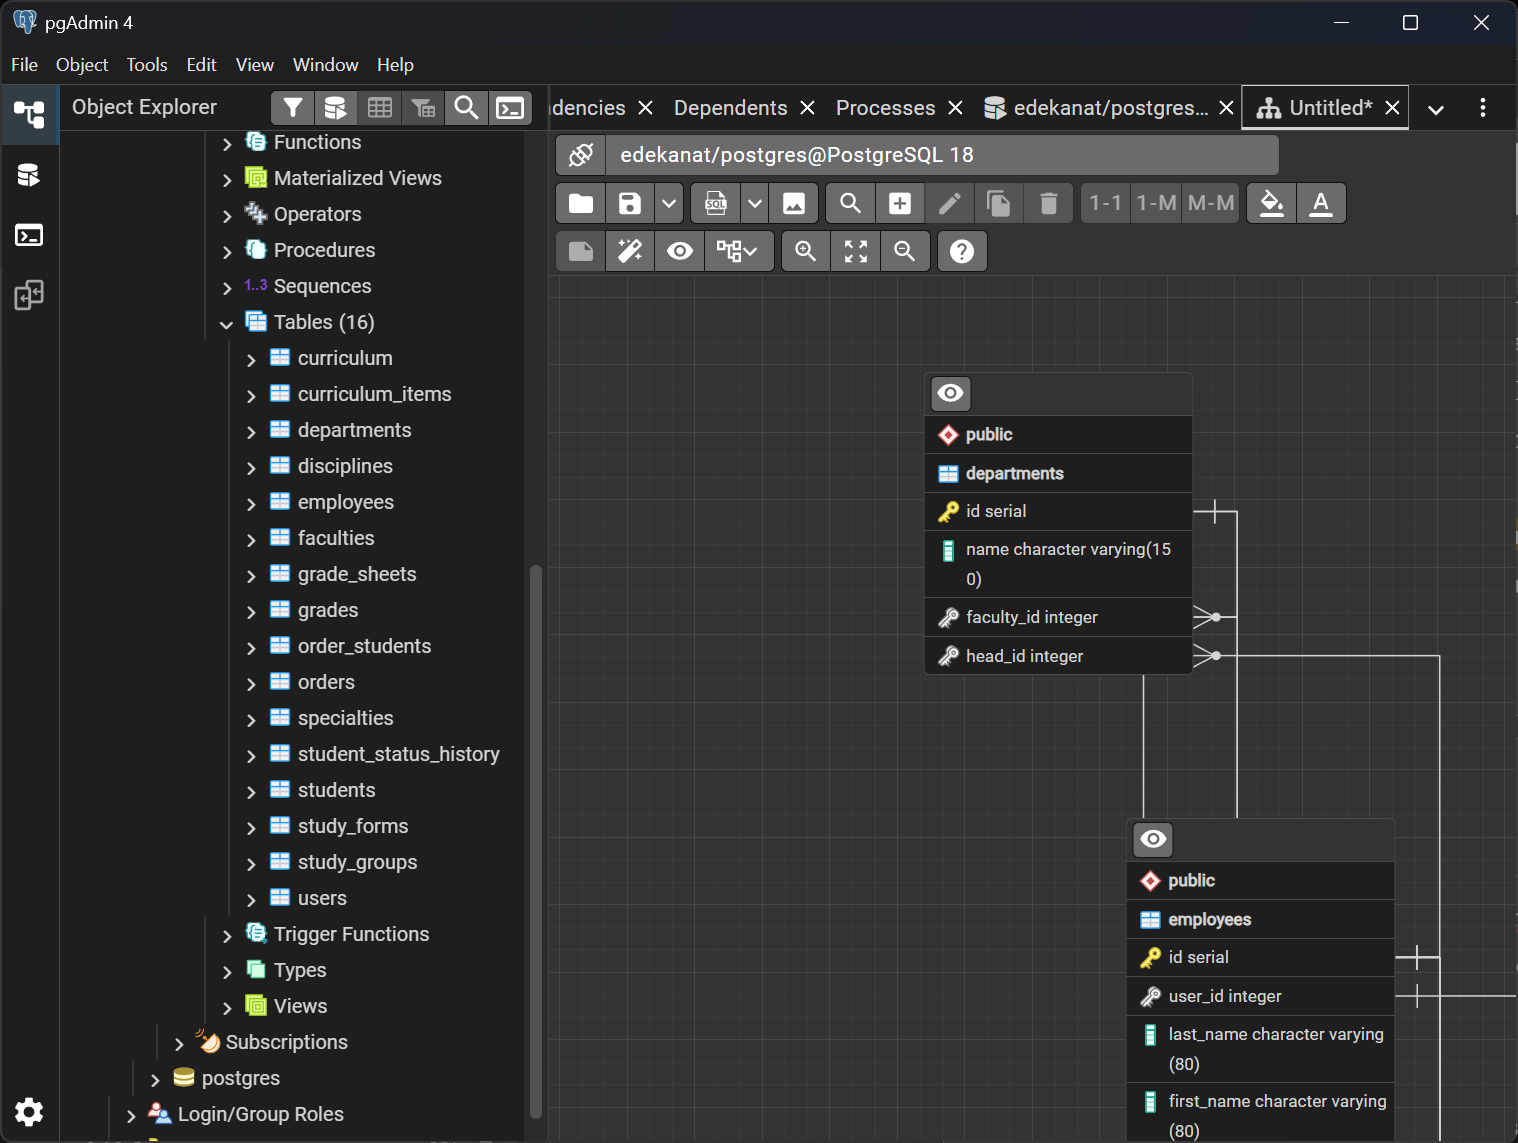
\includegraphics[width=0.9\textwidth]{media/image2.png}
\end{center}

\chapter{Приложение Б}
Скриншот Query Tool с выполненным запросом получения среднего балла студентов группы ПИ-101.

\vspace{0.5cm}
\begin{center}
    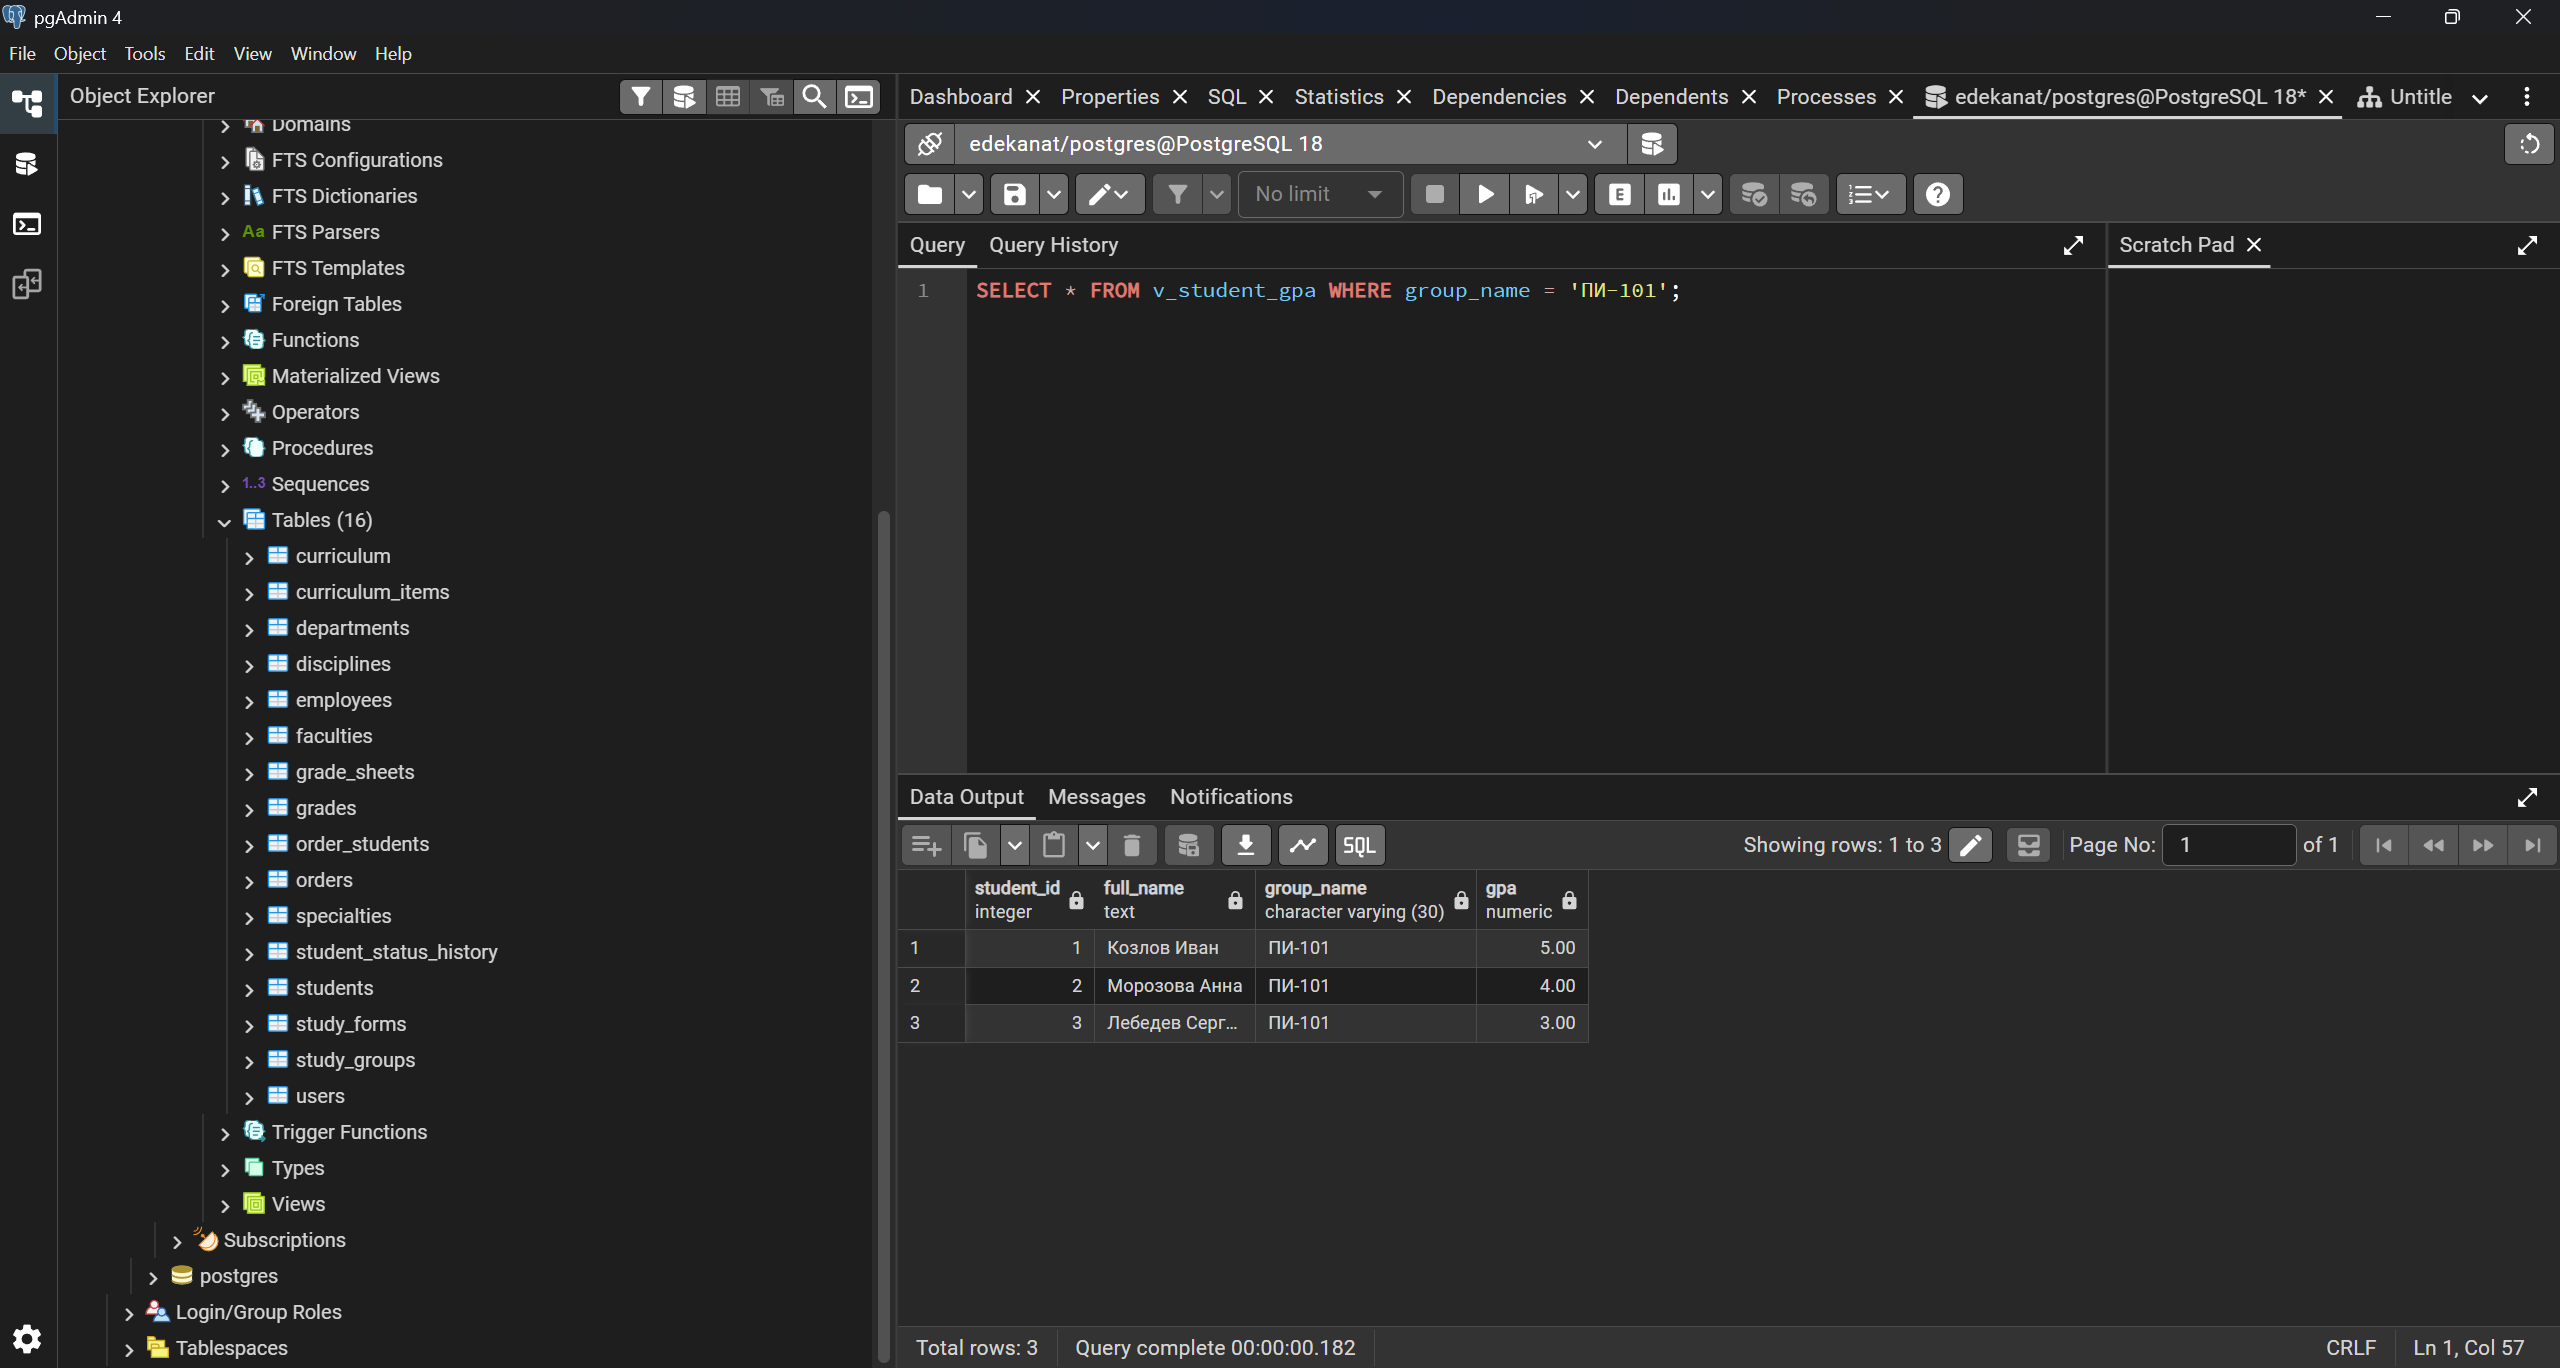
\includegraphics[width=0.9\textwidth]{media/image3.png}
\end{center}

\chapter{Приложение В}
Скриншот просмотра таблицы students в pgAdmin 4

\vspace{0.5cm}
\begin{center}
    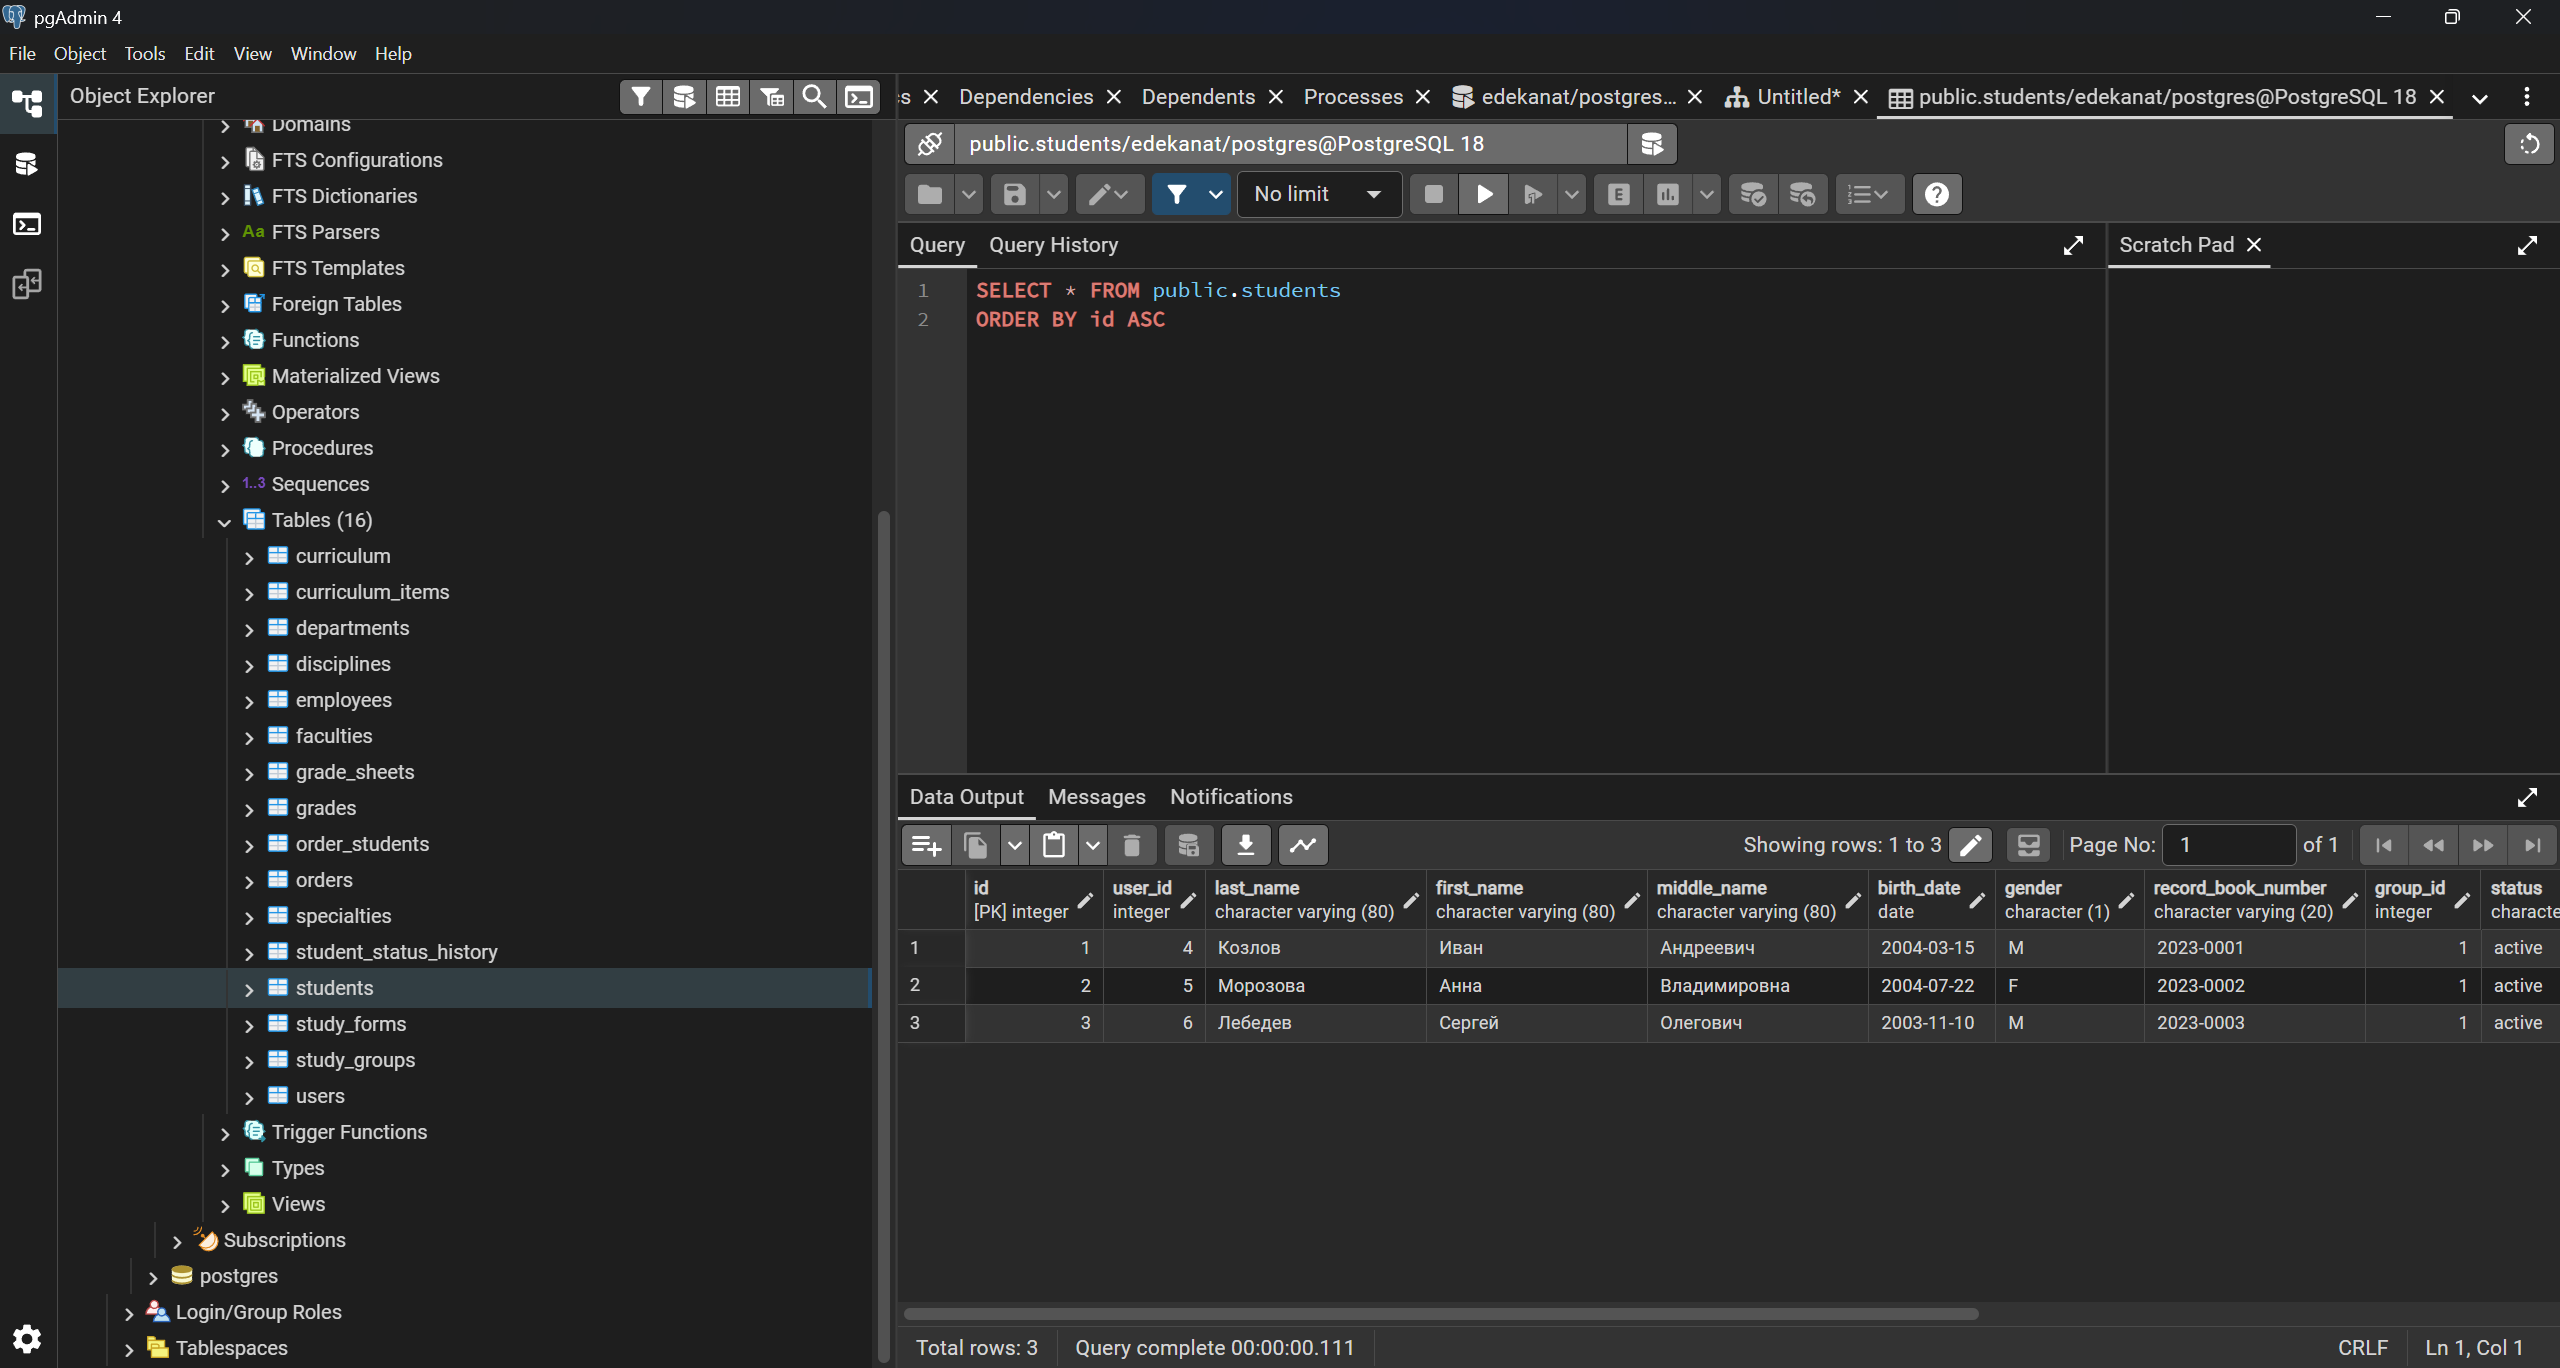
\includegraphics[width=0.9\textwidth]{media/image4.png}
\end{center}

\end{document}